\documentclass[border=10pt]{standalone}
\usepackage{pgfplots}
\pgfplotsset{compat=1.18}
\begin{document}
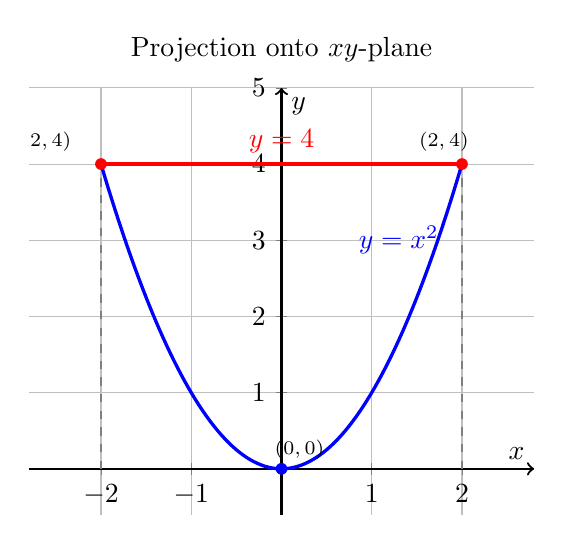
\begin{tikzpicture}
\begin{axis}[
    title={Projection onto $xy$-plane},
    xlabel={$x$}, ylabel={$y$},
    xmin=-2.8, xmax=2.8, ymin=-0.6, ymax=5,
    axis lines=middle, axis line style={->, thick},
    width=8cm, height=7cm,
    grid=both,
]
\addplot[blue, very thick, domain=-2:2, samples=100] {x^2};
\addplot[red, very thick] coordinates {(-2,4) (2,4)};
\addplot[gray, dashed, thin] coordinates {(-2,0) (-2,4)};
\addplot[gray, dashed, thin] coordinates {(2,0) (2,4)};
\node[blue] at (axis cs:1.3,3) {$y=x^2$};
\node[red] at (axis cs:0,4.3) {$y=4$};
\node[circle,fill=blue,inner sep=1.5pt] at (axis cs:0,0) {};
\node[circle,fill=red,inner sep=1.5pt] at (axis cs:-2,4) {};
\node[circle,fill=red,inner sep=1.5pt] at (axis cs:2,4) {};
\node at (axis cs:0.2,0.25) {\scriptsize$(0,0)$};
\node at (axis cs:-2.7,4.3) {\scriptsize$(-2,4)$};
\node at (axis cs:1.8,4.3) {\scriptsize$(2,4)$};
\end{axis}
\end{tikzpicture}
\end{document}